
\section{Evaluasi}
\subsection{Lingkungan Pengujian}

Kakas yang digunakan untuk testing adalah ApacheBench. Sesuai dengan namanya, ApacheBench dapat melakukan benchmarking pada web server. ApacheBench (ab) akan mengirim sejumlah request dan menghasilkan data kinerja web server yang dipilih. Data yang dihasilkan pleh ab diantaranya adalah jumlah byte yang dikirim antar web server dan ab, jumlah request per detik yang dapat ditangani server, waktu rata-rata yang digunakan untuk menangani sebuah request, serta waktu maksimum dan minimum yang digunakan dalam sebuah request.

Pengujian dilakukan pada \textit{cloud provider} DigitalOcean. Cloud dipilih karena proses pembuatan server on-demand dengan spesifikasi tertentu dapat dilakukan dengan mudah dan dalam waktu yang singkat. Penggunaan server dengan jumlah core yang tinggi yang dibutuhkan dapat dilakukan dengan menggunakan DigitalOcean CPU-Optimized Droplet. Droplet tersebut mendapatkan dedicated CPU sehingga komputasi paralel pada OpenSSL dapat berjalan dengan menggunakan CPU pada kapasitas maksimum. Arsitektur yang digunakan pada pengujian dapat dilihat pada Gambar \ref{fig:testing_arch}.

\begin{figure}[h]
  \centering
  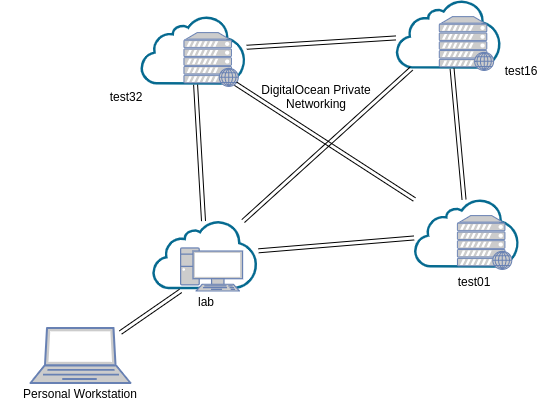
\includegraphics[width=0.8\textwidth]{resources/ch-4/testing_arch.png}
  \caption{Arsitektur Lingkungan Pengujian}
  \label{fig:testing_arch}
\end{figure}

Pengujian menggunakan empat Droplet, yaitu lab, test01, test16, dan test32. Setiap droplet terhubung melalui DigitalOcean Private Networking, dengan demikian latency antar droplet dapat dikurangi hingga seminimum mungkin. Droplet test01, test16, dan test32 merupakan droplet tempat diinstallnya Apache dan OpenSSL. Arsitektur aplikasi yang terinstall pada test01, test16, dan test32 sama dengan arsitektur implementasi pada Gambar \ref{fig:openssl_arch}. Droplet lab digunakan sebagai tempat melakukan testing dan tempat dijalankannya kakas ApacheBench. Komunikasi antar droplet lab dan personal workstation dilakukan dengan ssh.

\subsection{Skenario Pengujian}
Install apache, test pake apachebench, get waktu, rata2 tiga kali
\subsection{Hasil dan Analisis}
\subsubsection{Hasil Pengujian}
  Langsung data speedup aja, data raw simpen di lampiran

  \begin{table}[ht]
  \caption{Test table} % title of Table
  \centering % used for centering table
  \begin{tabular}{c c c c} % centered columns (4 columns)
  \hline\hline %inserts double horizontal lines
  Case & Method\#1 & Method\#2 & Method\#3 \\ [0.5ex] % inserts table
  %heading
  \hline % inserts single horizontal line
  1 & 50 & 837 & 970 \\ % inserting body of the table
  2 & 47 & 877 & 230 \\
  3 & 31 & 25 & 415 \\
  4 & 35 & 144 & 2356 \\
  5 & 45 & 300 & 556 \\ [1ex] % [1ex] adds vertical space
  \hline %inserts single line
  \end{tabular}
  \label{table:nonlin} % is used to refer this table in the text
  \end{table}

\subsubsection{Analisis Pengujian}
